Alexa ist der Name eines von der Firma Amazon entwickelten Voice Assistenten. Die verschiedenen Gerätevarianten sind jeweils mit mindestens einem Lautsprecher und sieben Mikrofonen ausgestattet. In Deutschland werden diese Geräte seit dem 26. Oktober 2016 angeboten. Durch die Mikrofone nimmt das Gerät die Geräusche in der Umgebung auf und versucht daraus die menschliche Sprache herauszufiltern. Dadurch bieten die Geräte die Funktionen eines Digitalen-Assistenten mittels Spracherkennung an, auch genannt Voice Assistant.
Alexa reagiert nicht dauerhaft auf gesagt Textpassagen sondern erst sobald ein aus einer beschränkten Auswahl gewähltes Wort genannt wird. Hier bietet Amazons Alexa folgende Aktivierungswörter an: Alexa, Echo, Amazon oder Computer. Sollte eines der Aktivierungswörter genannt werden beginnt ein LED-Indikator blau zu leuchten. Alles nun gesagte wird zur Erkennung an die Alexa Voice Services gesendet, wodurch auch sensible Daten über das Internet übertragen werden. Lediglich das erste Wort wird lokal verarbeitet, auch bietet das Gerät einen fest verlöteten Schalter um das Mikrofon zu deaktivieren. Dies wird über einen roten LED-Indikator angezeigt.\\

\subsection{Funktionen/Funktionsweise}
Mit Beginn der Einrichtung, beherrscht der VA bereits grundlegende Dinge wie: Wecker,Erinnerungen,Wetter abfrage, Internetsuche,Musik abspielen etc. . Diese sind immer gleich Aufgebaut. Mit dem mitteilen des "WakeWords" (z.B. Alexa oder Computer) wird der VA aktiviert und dann kann mittels des anschließend gesprochenem Textes die entsprechende Aktion ausgeführt werden. Mit "Alexa, stell meinen Wecker auf 6:30 Uhr" spricht man den Wecker-Skill an. Es gibt mittlerweile über 10.000 Skills welche auch von vielen Drittanbietern entwickelt werden. Außerdem kann man mit Alexa auch über den Online-Store von Amazon einkaufen.

\begin{figure}[H]
	\centering
	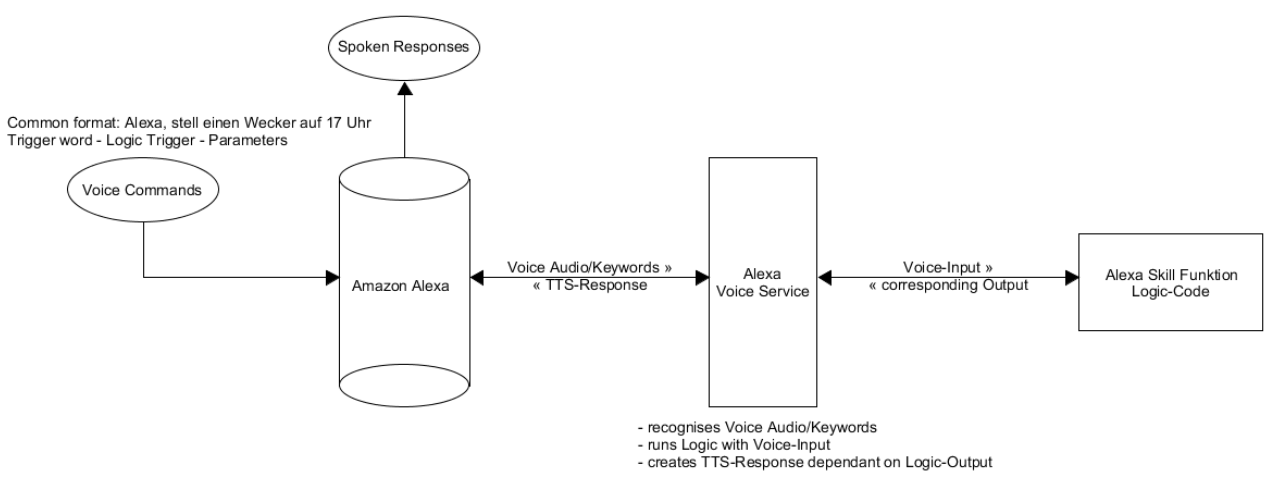
\includegraphics[width=0.9\textwidth]{content/img/AlexaVA_Architektur}
	\caption[Amazon Voice-Assistant Architektur]{Amazon Voice-Assistant Architektur}
\end{figure}

Oben wird die Struktur des VA als Diagramm gezeigt. Hier sieht man wie das Endgerät mit dem Alexa Voice Service kommuniziert und dieser dann alles entsprechend zusammenfügt und an die eigentliche Funktion übertragen. Diese verarbeitet dann die Abfrage und sendet eine Antwort zurück welche mittels TTS zu einer Stimme formatiert wird.

\subsection{Hardware}
Nachfolgend wird eine kleine Auswahl an Alexa-Geräten gezeigt. Insgesamt gibt es allerdings deutlich mehr.\\

Amazon Alexa Geräte:
\begin{itemize}
	\item Echo Spot (Alexa Lautsprecher mit kleinem Display)
	\item Echo Buttons ("Smart Home" Buttons)
	\item Echo Connect (Verbindet Alexa mit dem Telefon für Anrufe)
	\item Echo Show (7" Display - Anzeige von Videos und anderen Infos)
	\item Echo, Echo Dot und Echo Plus
	\item Alexa Sprachferbedienung (FireTV)
\end{itemize}

\subsubsection{Echo Dot (v2)}
\begin{figure}[H]
	\begin{minipage}{0.45\textwidth}
		\begin{itemize}
			\item 59,99€
			\item 7 Mikrofone - 1 Lautsprecher
			\item Hardwaretasten für die Lautstärke
			\item Arbeitet als Smart Home Hub
			\item ein Mute-Button für das Mikrofon auf dem Gerät
		\end{itemize}
	\end{minipage}
	\hfill
	\begin{minipage}{0.45\textwidth}
		\centering
		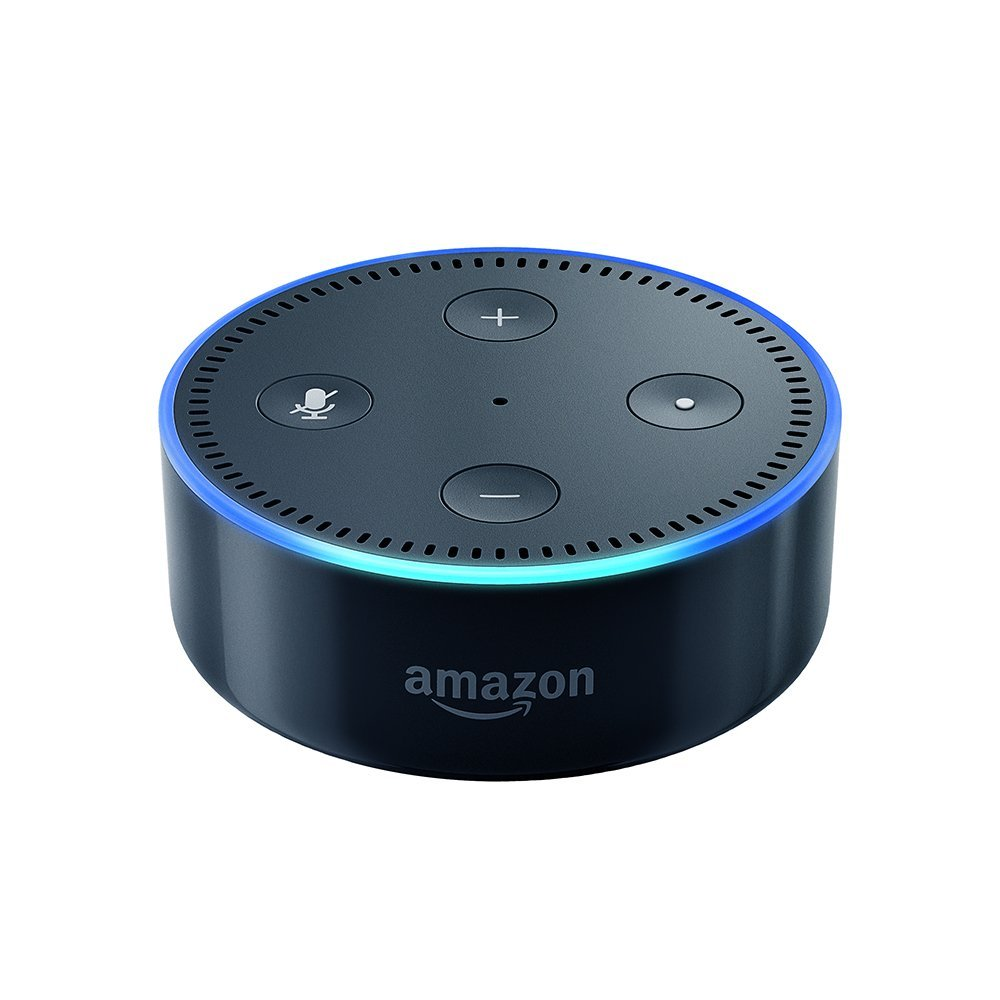
\includegraphics[width=\textwidth]{content/img/echodot}
		\caption[Echo Dot]{Echo Dot}
	\end{minipage}
\end{figure}

\subsubsection{Echo}
\begin{figure}[H]
	\begin{minipage}{0.45\textwidth}
		\begin{itemize}
			\item 99,99€
			\item Ähnlich wie Echo Dot
			\item Größere und bessere Lautsprecher
			\item 63mm-Woofer
			\item 16mm-Hochtonlautsprecher
		\end{itemize}
	\end{minipage}
	\hfill
	\begin{minipage}{0.45\textwidth}
		\centering
		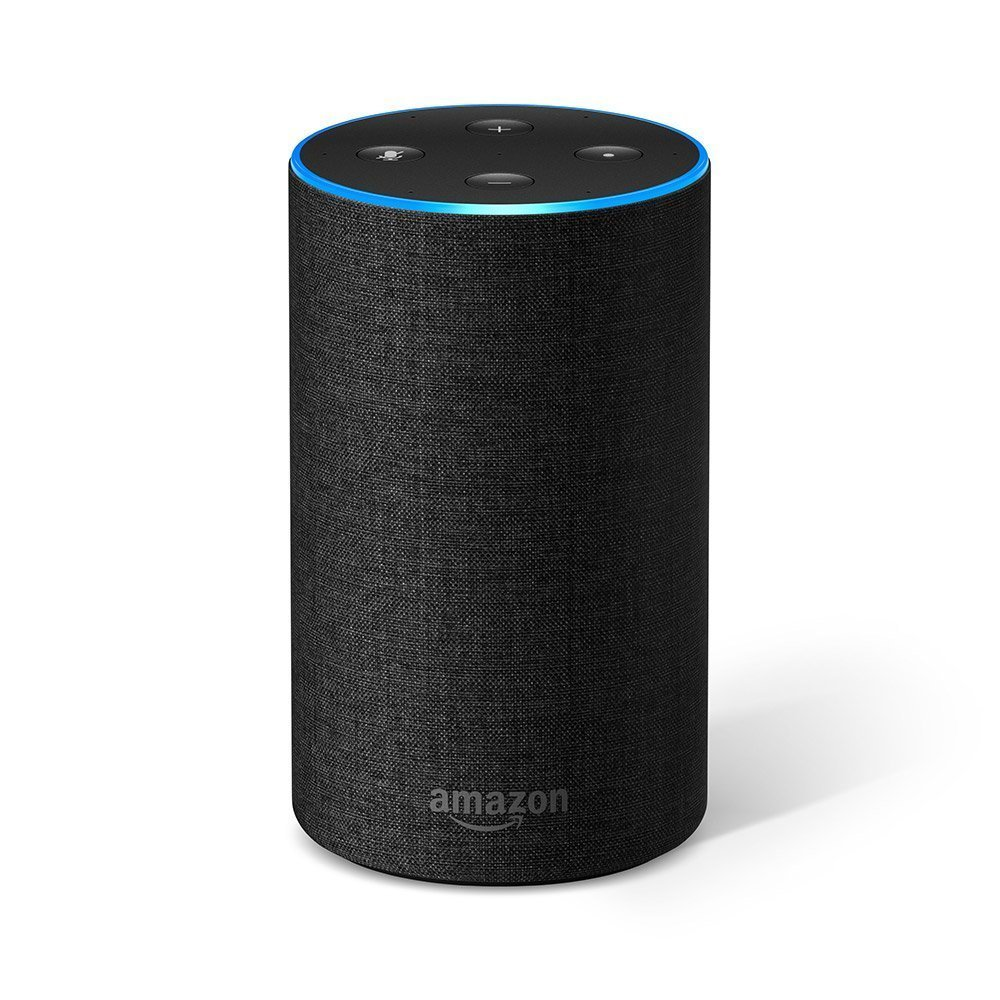
\includegraphics[width=\textwidth]{content/img/echo}
		\caption[Echo]{Echo}
	\end{minipage}
\end{figure}

\subsubsection{Echo Plus}
\begin{figure}[H]
	\begin{minipage}{0.45\textwidth}
		\begin{itemize}
			\item 149,99€
			\item Ähnlich wie Echo Dot und Echo
			\item integrierten ZigBee-Smart Home Hub
			\item Größere und bessere Lautsprecher
			\item 63mm-Woofer
			\item 20mm-Hochtonlautsprecher
		\end{itemize}
	\end{minipage}
	\hfill
	\begin{minipage}{0.45\textwidth}
		\centering
		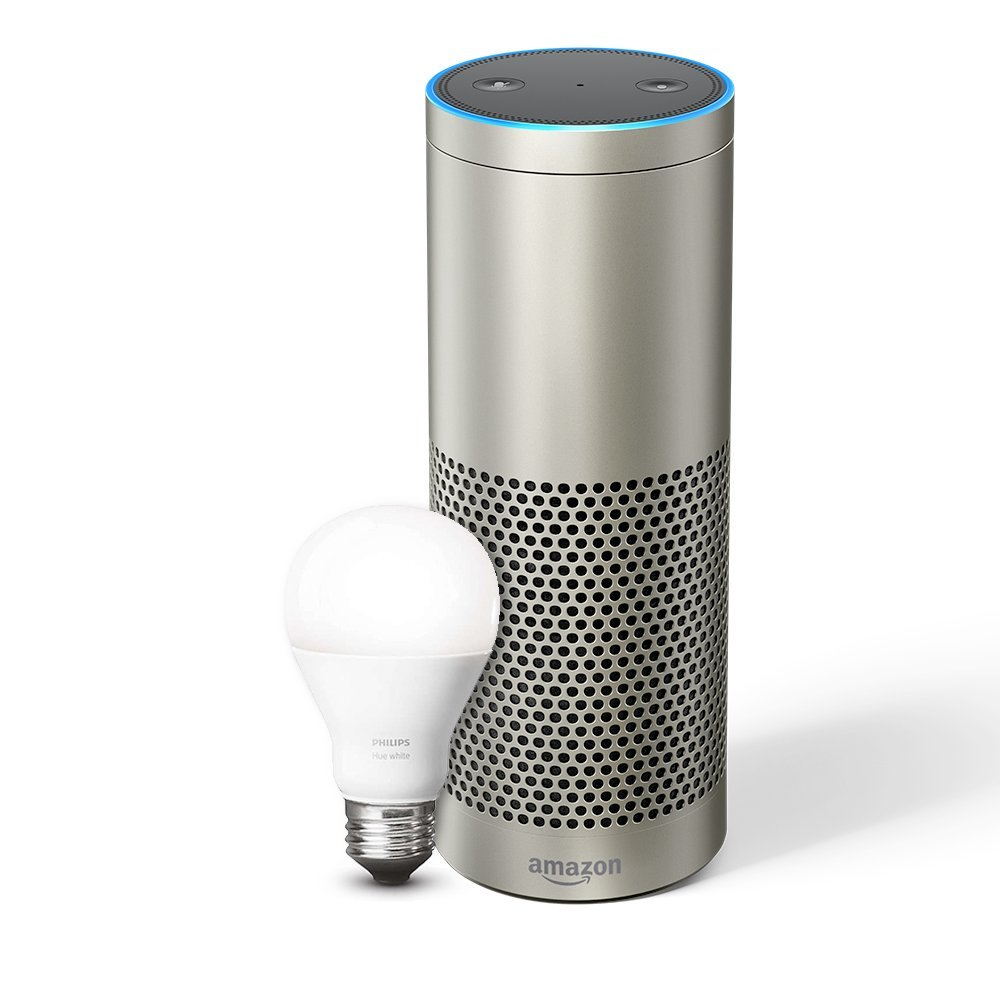
\includegraphics[width=\textwidth]{content/img/echoplus}
		\caption[Echo Plus]{Echo Plus}
	\end{minipage}
\end{figure}

\subsection{Erweiterbarkeit - Skills}
Der Alexa Skills Service bietet die Möglichkeit eigene Skills zu entwickeln und über den Store den anderen Nutzer bereitzustellen. Die Skills bedienen sich dabei einer Skills API, für welche es mittlerweile eine breite Unterstützung für viele verschiedene Programmier- und Skriptsprachen gibt. Jeder Skill verfolgt dabei ein festes Muster welches sich aus einem Dialogmuster, also einer Datei welche aussagt wie mit dem Nutzer kommuniziert wird und einer Funktion zusammensetzt. Diese Funktion wird in der Regel durch einen Webservice bereitgestellt, hierfür bietet sich der von Amazon bereitgestellte Service AWS Lambda an, da dieser bereits eine gute Integration in die Entwicklung darstellt.\\

Ein Skill besteht aus Utterances,Intents und einer Funktion. Utterances (auch Aussagen) werden einem Intent zugeordnet, der AVS nutzt diese um dem gesagten ein Intent zuzuweisen damit der korrekt Code ausgeführt wird. Ein paar Beispiele:
\begin{itemize}
	\item stell den Wecker
	\item wie spät ist es ?
	\item wann klingelt der Wecker ?
\end{itemize}
Diese zugeordneten Intents werden dann über einen eindeutigen Namen mit dem Code verknüpft. Im Code kann dann die entsprechende Antwort in Form eines Strings zurückgegeben werden.